\section{NP-hardness, polynomial cases, and exact exponential algorithm}
\label{sec:np}

In this section we focus on the classical complexity of the \textsc{$d$-Cut} problem, and on exact exponential algorithms. Namely, we provide the \NP-hardness result in Section~\ref{sec:NP-hard}, the polynomial algorithm for graphs of bounded degree in Section~\ref{sec:poly-algo}, and 
a simple exact exponential algorithm in Section~\ref{sec:exact-algo}.

\subsection{NP-hardness for regular graphs}
\label{sec:NP-hard}

Before stating our \NP-hardness result, we need some definitions and observations.

\begin{definition}
    A set of vertices $X \subseteq V(G)$ is said to be \emph{monochromatic} if, for any $d$-cut $(A, B)$ of $G$, $X \subseteq A$ or $X \subseteq B$.
\end{definition}

\begin{observation}
    \label{obs:mono_bipartite}
    For fixed every $d \geq 1$, if $u$ and $v$ have at least $2d+1$ common neighbors, the set $\{u,v\}$ is monochromatic.
    In particular, the graph $K_{d+1, 2d+1}$ is monochromatic.
    Moreover, if a vertex $v$ has at least $d+1$ neighbors in the monochromatic set $S$, $\{v\} \cup S$ is monochromatic.
\end{observation}

\begin{definition}[Spool]
    For $n,d \geq 1$, a \emph{$(d, n)$-spool}  is the graph obtained from $n$  copies of $K_{d+1, 2d+2}$ such that, for every $1 \leq i \leq n$, one vertex of degree $d+1$ of the $i$-th copy is identified with one vertex of degree $d+1$ of the $(i+1 \mod n)$-th copy, so that the two chosen vertices in each copy are distinct. %\ig{we need to say that, within each copy, the two ``identified'' vertices are distinct}.
    The \emph{exterior} vertices of a copy are those of degree $d+1$ that are not used to interface with another copy.
    The \emph{interior} vertices of a copy are those of degree $2d+2$ that do not interface with another copy.
\end{definition}

An illustration of a $(2,3)$-spool is shown in Figure~\ref{fig:spool}.

\begin{figure}[!htb]
    \centering
    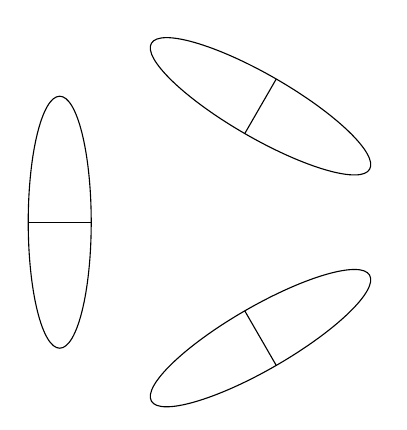
\begin{tikzpicture}[scale=1]
            %\draw[help lines] (-5,-5) grid (5,5);
            \GraphInit[unit=3,vstyle=Simple]
            \SetVertexSimple[Shape=circle, FillColor=black, MinSize=2pt]
            \tikzset{VertexStyle/.append style = {inner sep = \inners, outer sep = \outers}}
            \SetVertexNoLabel
            \foreach \x in {0,1,2} {
                \pgfmathtruncatemacro{\med}{(\x)*120 + 30}
                \begin{scope}[rotate=-\med]
                    \draw (0,1.7) ellipse (1.6cm and 0.4cm);
                    \draw (0,1.3) -- (0,2.1);
                \end{scope}
                \foreach \y in {0,1,2,3,4,5} {
                    \pgfmathtruncatemacro{\ang}{\x * 120 + \y * 24}
                    \Vertex[a=\ang, d=2]{i\x\y}
                }
                \foreach \y in {0,1,2} {
                    \pgfmathtruncatemacro{\ang}{\x * 120 + \y * 30 + 30}
                    \pgfmathsetmacro{\bla}{0.5 + mod(\y,2) *0.25}
                    \Vertex[a=\ang, d=\bla]{o\x\y}
                    \foreach \z in {0,1,2,3,4,5} {
                        \Edge(i\x\z)(o\x\y)
                    }
                }
            }
    \end{tikzpicture}
    \caption{A $(2,3)$-spool. Circled vertices are exterior vertices.\label{fig:spool}}
\end{figure}

\begin{observation}
    For fixed $d\geq 1$ and every $n \geq 1$, a $(d, n)$-spool is monochromatic.
\end{observation}




\begin{proof}
    Let $S$ be a $(d, n)$-spool.
    If $n=1$, the observation follows by combining the two statements of Observation~\ref{obs:mono_bipartite}.
    Now let $X, Y \subsetneq S$ be two copies of $K_{d+1,2d+2}$ that share exactly one vertex $v$.
    By Observation~\ref{obs:mono_bipartite}, $X' = X \setminus \{v\}$ and $Y' = Y \setminus \{v\}$ are monochromatic.
    Since $v$ has $d+1$ neighbors in $X'$ and $d+1$ in $Y'$, it follows that $X \cup Y$ is monochromatic. By repeating the same argument for every  two copies of $K_{d+1,2d+2}$ that share exactly one vertex, the observation follows.
\end{proof}


\cite{chvatal_matching_cut} proved that \textsc{Matching Cut} is \NP-hard for graphs of maximum degree at least four. In the next theorem, whose proof is inspired by the reduction of \cite{chvatal_matching_cut}, we prove the \NP-hardness of \pname{$d$-cut} for $(2d+2)$-regular graphs. In particular, for $d=1$ it implies the \NPHness\ of \pname{Matching Cut} for $4$-regular graphs.


\begin{theorem}
    \label{thm:regular_nph}
    For every integer $d \geq 1$, \pname{$d$-cut} is \NP-hard even when restricted to $(2d+2)$-regular graphs.
\end{theorem}

%\ig{IMPORTANT: the degree bound $(2d+2)$ is unlikely to be improved, in the following sense: if we had an \NP-hardness result for  $(2d+1)$-regular graphs, this would disprove the conjecture about the existence of internal partitions on $r$-regular graphs~\cite{internal_partition_regular6}, for $r$ odd, unless all the problems in $\NP$ could be solved in {\sl constant} time}

\begin{proof}
    Our reduction is from the \pname{3-Uniform Hypergraph Bicoloring} problem, which is \NP-hard; see~\cite{lovasz_hypergraph}. %\ig{Say that this reduction is strongly inspired by~\cite{chvatal_matching_cut}!}

    \problem{3-Uniform Hypergraph Bicoloring}{A hypergraph $\mathcal{H}$ with exactly three vertices in each hyperedge.}{Can we 2-color $V(\mathcal{H})$ such that no hyperedge is monochromatic?}

    Throughout this proof, $i$ is an index representing a color, $j$ and $k$ are redundancy indices used to increase the degree of some sets of vertices, and $\ell$ and $r$ are indices used to refer to separations of sets of exterior vertices.

    Given an instance $\mathcal{H}$ of \pname{3-Uniform Hypergraph Bicoloring}, we proceed to construct a $(2d+2)$-regular instance $G$ of \pname{$d$-Cut} as follows. For each vertex $v \in V(\mathcal{H})$, add a $(d,4\dgr(v) + 1)$-spool to $G$.
    Each set of exterior vertices receives an (arbitrarily chosen) unique label from the following types: $S(v^*)$ and $S(v, e, i, j)$, such that $i,j \in [2]$ and $e \in E(\mathcal{H})$ with $v \in e$.
    Separate each of the labeled sets into two parts of equal size (see Figure~\ref{fig:spool}).
    For the first type, we denote the sets by $S(v^*, i)$, $i \in [2]$; for the second type, by $S_{\ell}(v, e, i, j)$, $\ell \in [2]$.
    For each set $S(v^*, i)$, we choose an arbitrary vertex and label it with $s(v^*, i)$.
    To conclude the construction of vertex gadgets, add every edge between $S_1(v, e, i, j)$ and $S_2(v, e, i, j)$, and form a perfect matching between $S(v^*, 1) \setminus \{s(v^*, 1)\}$ and $S(v^*, 2) \setminus \{s(v^*, 2)\}$.
    Note that all inner vertices of a spool have degree $2d+2$, every vertex labeled $s(v^*, i)$ has $d+1$ neighbors, every other vertex in $S(v^*, i)$ has $d+2$, and every vertex in $S(v, e, i, j)$ has degree equal to $2d+1$.
    For an example of the edges between exterior vertices of the same vertex gadget, see Figure~\ref{fig:vert_relations}.

    \begin{figure}[!htb]
        \centering
        \hspace*{-0.2cm}\begin{tikzpicture}[scale=1]
            \begin{scope}[shift={(0cm,0)}]
                %\draw[help lines] (0,-5) grid (12,5);
                \GraphInit[unit=3,vstyle=Normal]
                \SetVertexNormal[Shape=circle, FillColor=black, MinSize=2pt]
                \tikzset{VertexStyle/.append style = {inner sep = \inners, outer sep = \outers}}
                \pgfmathtruncatemacro{\zero}{0}
                \pgfmathtruncatemacro{\one}{1}
                \pgfmathtruncatemacro{\six}{6}
                    \foreach \w in {1} {
                        \foreach \x in {0,1} {
                            \foreach \y in {1,2,3,4,5,6} {
                                \pgfmathsetmacro{\bla}{(6.0 + 12.0/7.0) * \x + 5.0/7.0 * \y}
                                \pgfmathsetmacro{\bly}{-3 * \w}
                                \pgfmathtruncatemacro{\wo}{\w + 1}
                                \ifnum\x=\zero
                                    \Vertex[x=\bla, y=\bly, NoLabel]{e\w\x\y}
                                \else
                                    \ifnum\y=\one
                                        \Vertex[x=\bla, y=\bly, Math, LabelOut, Ldist=-4pt,Lpos=180,L={s(v^*, 1)}]{e\w\x\y}
                                    \else
                                        \ifnum\y=\six
                                          \Vertex[x=\bla, y=\bly, Math, LabelOut, Ldist=1pt,Lpos=0,L={s(v^*, 2)}]{e\w\x\y}
                                        \else
                                            \Vertex[x=\bla, y=\bly, NoLabel]{e\w\x\y}
                                        \fi
                                    \fi
                                \fi
                            }
                            \pgfmathsetmacro{\bla}{2.5 + (6.0 + 12.0/7.0) * \x}
                            \pgfmathsetmacro{\blam}{\bla - 1.2}
                            \pgfmathsetmacro{\blap}{\bla + 1.2}
                            \ifnum\w=\zero
                                \draw (\bla,-0.7) -- (\bla,1.2);
                            \else
                                \draw (\bla,-4.2) -- (\bla,-2.3);
                            \fi
                            \ifnum\w=\zero
                                \ifnum\x=\zero
                                    \node at (\blam,1) {$S_1(v, e, i, 1)$};
                                    \node at (\blap,1) {$S_2(v, e, i, 1)$};
                                \else
                                    \node at (\blam,1) {$S_1(v^*, 1)$};
                                    \node at (\blap,1) {$S_2(v^*, 1)$};
                                \fi
                            \else
                                \ifnum\x=\zero
                                    \node at (\blam,-4) {$S_1(v, e, i, 2)$};
                                    \node at (\blap,-4) {$S_2(v, e, i, 2)$};
                                \else
                                    \node at (\blam,-4) {$S(v^*, 1)$};
                                    \node at (\blap,-4) {$S(v^*, 2)$};
                                \fi
                            \fi
                        }
                    \foreach \z in {4,5,6} {
                        \Edge[style = bend left](e\w01)(e\w0\z)
                        \Edge[style = bend right](e\w02)(e\w0\z)
                    }
                    \Edge(e\w03)(e\w04)
                    \Edge[style = bend left](e\w03)(e\w05)
                    \Edge[style = bend left](e\w03)(e\w06)
                    \Edge[style = bend left](e\w12)(e\w15)
                    \Edge(e\w13)(e\w14)
                }
            \end{scope}
        \end{tikzpicture}
        \caption{Relationships between exterior vertices of a vertex gadget ($d=3$).\label{fig:vert_relations}}
    \end{figure}

    For each color $i \in [2]$, add a $(d, n + 2m)$-spool to $G$, where $n = |V(\mathcal{H})|$ and $m = |E(\mathcal{H})|$.
    Much like the exterior vertices of the vertex gadgets, we attribute unique labels: $C(v, i)$, for each $v \in V(\mathcal{H})$, and $C(e, i, j)$, for each $e \in E(\mathcal{H})$ and $j \in [2]$.
    Now, split the remaining vertices of each labeled set into two equal-sized parts $C_1(\cdot), C_2(\cdot)$ and label one vertex of each $C_{\ell}(e, i, j)$ with the label $c_{\ell}(e, i, j)$ and one of each $C_{\ell}(v, i)$ with $c_{\ell}(v,i)$.
    To conclude, add all edges from $c_{\ell}(v, i)$ to $C_{\ell}(v, i)$, add the edge $c_{\ell}(v, i)c_{3-\ell}(v, i)$, make each $C_{\ell}(e, i, j) \setminus \{c_{\ell}(e, i, j)\}$ into a clique, and, between $C_{\ell}(e, i, j) \setminus \{c_{\ell}(e, i, j)\}$ and $C_r(e, i, k) \setminus \{c_r(e, i, k)\}$, add edges to form a perfect matching, for $\ell,j,r,k \in [2]$.
    That is, each $C_{\ell}(e, i, j)$ forms a perfect matching with three other sets of exterior vertices.
    So far, each $c_{\ell}(v, i)$ has degree $(d+1) + (d-1) + 1 = 2d+1$, other vertices of $C_{\ell}(v, i)$ have degree $d+2$, each vertex in $C_{\ell}(e, i, j) \setminus \{c_{\ell}(e, i, j)\}$ has degree $(d + 1) + (d - 2) + 3 = 2d + 2$, and each vertex labeled $c_{\ell}(e, i, j)$ has degree $d + 1$.

    We now add edges between vertices of different color gadgets.
    In particular, we add every edge between $C_1(v, 2) \setminus \{c_1(v, 2)\}$ and $C_2(v, 1) \setminus \{c_2(v, 1)\}$.
    This increases the degree of these vertices to $2d+1$.
    An example when $d=3$ is illustrated in Figure~\ref{fig:color_relations}.

    \begin{figure}[!htb]
        \centering
        \hspace*{-1cm}\begin{tikzpicture}[scale=1]
            \begin{scope}[shift={(0cm,0)}]
                %\draw[help lines] (0,-5) grid (12,5);
                \GraphInit[unit=3,vstyle=Normal]
                \SetVertexNormal[Shape=circle, FillColor=black, MinSize=2pt]
                \tikzset{VertexStyle/.append style = {inner sep = \inners, outer sep = \outers}}
                \pgfmathtruncatemacro{\zero}{0}
                \pgfmathtruncatemacro{\one}{1}
                \pgfmathtruncatemacro{\six}{6}
                    \foreach \w in {0, 1} {
                        \foreach \x in {0,1} {
                            \foreach \y in {1,2,3,4,5,6} {
                                \pgfmathsetmacro{\bla}{(6.0 + 12.0/7.0) * \x + 5.0/7.0 * \y}
                                \pgfmathsetmacro{\bly}{-3 * \w}
                                \pgfmathtruncatemacro{\wo}{\w + 1}
                                \ifnum\x=\zero
                                   \ifnum\y=\one
                                    \Vertex[x=\bla, y=\bly, Math, LabelOut, Lpos=180, Ldist=-2pt, L={c_1(e,i,\wo)}]{e\w\x\y}
                                   \else
                                       \ifnum\y=\six
                                           \Vertex[x=\bla, y=\bly, Math, LabelOut, Lpos=-45, Ldist=-2pt, L={c_2(e,i,\wo)}]{e\w\x\y}
                                       \else
                                        \Vertex[x=\bla, y=\bly, NoLabel]{e\w\x\y}
                                       \fi
                                    \fi
                                \else
                                    \ifnum\w=\one
                                       \ifnum\y=\one
                                        \Vertex[x=\bla, y=\bly, Math, LabelOut, Lpos=135, Ldist=-2pt, L={c_1(v,2)}]{e\w\x\y}
                                       \else
                                           \ifnum\y=\six
                                               \Vertex[x=\bla, y=\bly, Math, LabelOut, Lpos=0, Ldist=-2pt, L={c_{2}(v, 2)}]{e\w\x\y}
                                           \else
                                            \Vertex[x=\bla, y=\bly, NoLabel]{e\w\x\y}
                                           \fi
                                        \fi
                                    \else
                                        \ifnum\y=\one
                                        \Vertex[x=\bla, y=\bly, Math, LabelOut, Lpos=135, Ldist=-2pt, L={c_1(v,1)}]{e\w\x\y}
                                       \else
                                           \ifnum\y=\six
                                               \Vertex[x=\bla, y=\bly, Math, LabelOut, Lpos=0, Ldist=-2pt, L={c_{2}(v, 1)}]{e\w\x\y}
                                           \else
                                            \Vertex[x=\bla, y=\bly, NoLabel]{e\w\x\y}
                                           \fi
                                        \fi
                                    \fi
                                \fi
                            }
                            \ifnum\x=\zero
                                \Edge(e\w\x2)(e\w\x3)
                                \Edge(e\w\x4)(e\w\x5)
                                \ifnum\w=\zero
                                    \Edge[style=bend left](e\w\x2)(e\w\x5)
                                    \Edge[style=bend left](e\w\x3)(e\w\x4)
                                \else
                                    \Edge[style=bend right](e\w\x2)(e\w\x5)
                                    \Edge[style=bend right](e\w\x3)(e\w\x4)
                                \fi
                            \else
                                \newcommand{\bla}{right}
                                \ifnum\w=\zero
                                    \renewcommand{\bla}{left}
                                \fi

                                \foreach \y in {2,3} {
                                    \pgfmathtruncatemacro{\z}{7 - \y}
                                    \Edge[style=bend \bla](e\w\x1)(e\w\x\y)
                                    \Edge[style=bend \bla](e\w\x\z)(e\w\x6)
                                    \Edge[style=bend \bla](e\w\x1)(e\w\x6)
                                }
                            \fi
                            \pgfmathsetmacro{\bla}{2.5 + (6.0 + 12.0/7.0) * \x}
                            \pgfmathsetmacro{\blam}{\bla - 1.2}
                            \pgfmathsetmacro{\blap}{\bla + 1.2}
                            \ifnum\w=\zero
                                \draw (\bla,-0.7) -- (\bla,1.2);
                            \else
                                \draw (\bla,-4.2) -- (\bla,-2.3);
                            \fi
                            \ifnum\w=\zero
                                \ifnum\x=\zero
                                    \node at (\blam,1) {$C_1(e, i, 1)$};
                                    \node at (\blap,1) {$C_2(e, i, 1)$};
                                \else
                                    \node at (\blam,1) {$C_1(v, 1)$};
                                    \node at (\blap,1) {$C_2(v, 1)$};
                                \fi
                            \else
                                \ifnum\x=\zero
                                    \node at (\blam,-4) {$C_1(e, i, 2)$};
                                    \node at (\blap,-4) {$C_2(e, i, 2)$};
                                \else
                                    \node at (\blam,-4) {$C_1(v, 2)$};
                                    \node at (\blap,-4) {$C_2(v, 2)$};
                                \fi
                            \fi
                        }
                }
                \foreach \y in {2,3,4,5} {
                    \Edge(e00\y)(e10\y)
                }
                \foreach \y in {2,3} {
                    \pgfmathtruncatemacro{\yp}{\y+2}
                    \pgfmathtruncatemacro{\ym}{7 - \y}
                    \Edge(e00\y)(e10\yp)
                    \Edge(e10\y)(e00\yp)
                    \foreach \z in {4,5} {
                        \Edge(e11\y)(e01\z)
                    }
                }
            \end{scope}
        \end{tikzpicture}
        \caption{Relationships between exterior vertices of color gadgets ($d=3$).\label{fig:color_relations}}
    \end{figure}

    As a first step to connect color gadgets and vertex gadgets, we add every edge between $s(v^*, i)$ and $C_i(v, i)$, every edge between $S(v^*, i) \setminus \{s(v^*, i)\}$ and $C_i(v, i) \setminus \{c_{i}(v, i)\}$, a perfect matching between $S(v^*, i) \setminus \{s(v^*, i)\}$ and $C_{3-i}(v, i) \setminus \{c_{3-i}(v, i)\}$, and the edge $s(v^*, i)c_i(v, 3-i)$.
    Note that this last edge is fundamental, not only because it increases the degrees to the desired value, but also because, if both color gadgets belong to the same side of the cut, every $s(v^*, i)$ will have the same color and, since spools are monochromatic, so would be the \textit{entire} graph, as discussed in more detail below.
    Also note that, aside from $s(v^*, i)$, no other vertex has more than $d$ neighbors outside of its spool.
    The edges described in this paragraph increase the degree of every $s(v^*, i)$ by $d + 1$, yielding a total degree of $2d+2$, of every vertex in $S(v^*, i) \setminus \{s(v^*, i)\}$ to $(d+2) + (d-1) + 1 = 2d+2$, of every vertex in $C_{i}(v, i) \setminus \{c_i(v, i)\}$ to $(d+2) + d = 2d+2$, of every vertex in $C_{i}(v, 3-i) \setminus \{c_i(v, 3-i)\}$ to $(2d+1) + 1 = 2d+2$, and of every $c_{\ell}(v, i)$ to $(2d+1) + 1 = 2d+2$.
    Figure~\ref{fig:color_vertex_relations} gives an example of these connections.


    \begin{figure}[!htb]
        \centering
        \hspace*{-1cm}\begin{tikzpicture}[scale=1]
            \begin{scope}[shift={(0cm,0)}]
                %\draw[help lines] (0,-5) grid (12,5);
                \GraphInit[unit=3,vstyle=Normal]
                \SetVertexNormal[Shape=circle, FillColor=black, MinSize=2pt]
                \tikzset{VertexStyle/.append style = {inner sep = \inners, outer sep = \outers}}
                \pgfmathtruncatemacro{\zero}{0}
                \pgfmathtruncatemacro{\one}{1}
                \pgfmathtruncatemacro{\six}{6}
                    \foreach \w in {0, 1} {
                        \foreach \x in {1} {
                            \foreach \y in {1,2,3,4,5,6} {
                                \pgfmathsetmacro{\bla}{(6.0 + 12.0/7.0) * \x + 5.0/7.0 * \y}
                                \pgfmathsetmacro{\bly}{-3 * \w}
                                \pgfmathtruncatemacro{\wo}{\w + 1}
                                \ifnum\x=\zero
                                \else
                                    \ifnum\w=\one
                                       \ifnum\y=\one
                                        \Vertex[x=\bla, y=\bly, Math, LabelOut, Lpos=135, Ldist=-2pt, L={s(v^*,1)}]{e\w\x\y}
                                       \else
                                           \ifnum\y=\six
                                               \Vertex[x=\bla, y=\bly, Math, LabelOut, Lpos=0, Ldist=-2pt, L={c_{1}(v, 2)}]{e\w\x\y}
                                           \else
                                            \Vertex[x=\bla, y=\bly, NoLabel]{e\w\x\y}
                                           \fi
                                        \fi
                                    \else
                                        \ifnum\y=\one
                                        \Vertex[x=\bla, y=\bly, Math, LabelOut, Lpos=135, Ldist=-2pt, L={c_1(v,1)}]{e\w\x\y}
                                       \else
                                           \ifnum\y=\six
                                               \Vertex[x=\bla, y=\bly, Math, LabelOut, Lpos=0, Ldist=-2pt, L={c_{2}(v, 1)}]{e\w\x\y}
                                           \else
                                            \Vertex[x=\bla, y=\bly, NoLabel]{e\w\x\y}
                                           \fi
                                        \fi
                                    \fi
                                \fi
                            }
                            \ifnum\x=\zero
                                \Edge(e\w\x2)(e\w\x3)
                                \Edge(e\w\x4)(e\w\x5)
                                \ifnum\w=\zero
                                    \Edge[style=bend left](e\w\x2)(e\w\x5)
                                    \Edge[style=bend left](e\w\x3)(e\w\x4)
                                \else
                                    \Edge[style=bend right](e\w\x2)(e\w\x5)
                                    \Edge[style=bend right](e\w\x3)(e\w\x4)
                                \fi
                            \else
                                \newcommand{\bla}{right}
                                \ifnum\w=\zero
                                    \renewcommand{\bla}{left}
                                \fi
                                 \foreach \y in {2,3} {
                                     \pgfmathtruncatemacro{\z}{7 - \y}
                                     \ifnum\w=\zero
                                         \Edge[style=bend \bla](e\w\x1)(e\w\x\y)
                                     \fi
                                    \Edge[style=bend \bla](e\w\x1)(e\w\x6)
                                     \Edge[style=bend \bla](e\w\x\z)(e\w\x6)
                                 }
                            \fi
                            \pgfmathsetmacro{\bla}{2.5 + (6.0 + 12.0/7.0) * \x}
                            \pgfmathsetmacro{\blam}{\bla - 1.2}
                            \pgfmathsetmacro{\blap}{\bla + 1.2}
                            \ifnum\w=\zero
                                \draw (\bla,-0.7) -- (\bla,1.2);
                            \else
                                \draw (\bla,-4.2) -- (\bla,-2.3);
                            \fi
                            \ifnum\w=\zero
                                \ifnum\x=\zero
                                \else
                                    \node at (\blam,1) {$C_1(v, 1)$};
                                    \node at (\blap,1) {$C_2(v, 1)$};
                                \fi
                            \else
                                \ifnum\x=\zero
                                \else
                                    \node at (\blam,-4) {$S(v^*, 1)$};
                                    \node at (\blap,-4) {$C_1(v, 2)$};
                                \fi
                            \fi
                        }
                }
                \Edge(e111)(e011)
                \foreach \y in {1,2,3} {
                    \foreach \z in {2,3} {
                        \Edge(e11\y)(e01\z)
                    }
                }
                \foreach \y in {4,5} {
                    \pgfmathtruncatemacro{\ym}{\y - 2}
                    \Edge(e11\ym)(e01\y)
                    \foreach \z in {4,5} {
                        \Edge(e11\y)(e01\z)
                    }
                }
            \end{scope}
        \end{tikzpicture}
        \caption{Relationships between exterior vertices of color and vertex gadgets ($d=3$).\label{fig:color_vertex_relations}}
    \end{figure}



    For the final group of gadgets, namely hyperedge gadgets, for each $\{x, y, z\} \in E(\mathcal{H})$, each color $i$, and each pair $j,\ell \in [2]$, we add one additional vertex $c_{\ell}'(e, i, j)$ adjacent to $c_{\ell}(e, i, j)$, $S_{\ell}(x, e, i, j)$, $S_{\ell}(y, e, i , j)$, and $c_{3-\ell}'(e, i, j)$; finally, we add every edge between $c_{\ell}(e, i, j)$ and $S_{\ell}(z, e, i ,j)$. See Figure~\ref{fig:hyper_relations} for an illustration.
    Note that $c_{\ell}'(e, i, j)$ has degree $2d + 2$; the degree of $c_{\ell}(e, i ,j)$ increased from $d + 1$ to $2d + 2$, and the degree of each vertex of $S_{\ell}(x, e, i, j)$ increased from $2d + 1$ to $2d + 2$.
    This concludes our construction of the $(2d + 2)$-regular graph $G$.

    \begin{figure}[!htb]
        \centering
        \hspace*{-0.25cm}\begin{tikzpicture}[scale=1]
            \begin{scope}[shift={(0cm,0)}]
                %\draw[help lines] (0,-5) grid (12,5);
                \GraphInit[unit=3,vstyle=Normal]
                \SetVertexNormal[Shape=circle, FillColor=black, MinSize=2pt]
                \tikzset{VertexStyle/.append style = {inner sep = \inners, outer sep = \outers}}
                \pgfmathtruncatemacro{\zero}{0}
                \pgfmathtruncatemacro{\one}{1}
                \pgfmathtruncatemacro{\six}{6}
                \foreach \x in {0,1} {
                    \pgfmathtruncatemacro{\sh}{(6.29 + 12.0/7.0) * \x}
                    \begin{scope}[shift={(\sh,0)}]
                        \pgfmathtruncatemacro{\xp}{1 + 1*\x}
                        \pgfmathtruncatemacro{\pe}{180*(\x)}
                        \pgfmathtruncatemacro{\pep}{45 + 90*(1-\x)}
                        \Vertex[x=0, y=1.1, Math, LabelOut, Ldist=-2pt,Lpos=\pe,L={c_\xp(e,i,j)}]{e\x}
                        \Vertex[x=0, y=0.2, Math, LabelOut, Ldist=-2pt,Lpos=\pep,L={c'_\xp(e,i,j)}]{ep\x}
                        \Edge(e\x)(ep\x)
                        \foreach \w in {0,1,2} {
                            \pgfmathsetmacro{\ang}{120*(\w+1)}
                            \begin{scope}[rotate=\ang]
                                \foreach \y in {1,2,3} {
                                    \pgfmathsetmacro{\gap}{5.0/8.0}
                                    \pgfmathsetmacro{\bla}{\gap * \y - 2*\gap}
                                    \pgfmathtruncatemacro{\ym}{\y - 1}
                                    \newcommand{\setname}{z}
                                    \newcommand{\lpos}{270}
                                    \newcommand{\ldist}{13pt}
                                    \ifnum\w>\one
                                        \renewcommand{\lpos}{90}
                                        \renewcommand{\ldist}{0pt}
                                    \fi
                                    \ifnum\w=\zero
                                        \renewcommand{\setname}{x}
                                    \fi
                                    \ifnum\w=\one
                                        \renewcommand{\setname}{y}
                                    \fi
                                    \ifnum\ym=\one
                                        \Vertex[x=\bla, y=1.8, Math, LabelOut, Lpos=\lpos, Ldist=\ldist, L={S_{\xp}(\setname, e, i, j)}]{e\w\x\y}
                                    \else
                                        \Vertex[x=\bla, y=1.8, NoLabel]{e\w\x\y}
                                    \fi
                                    \ifnum\w>\one
                                        \Edge(e\x)(e\w\x\y)
                                    \else
                                        \Edge(ep\x)(e\w\x\y)
                                    \fi
                                }
                            \end{scope}
                        }
                    \end{scope}
                }
                \Edge(ep0)(ep1)
            \end{scope}
        \end{tikzpicture}
        \caption{Hyperedge gadget ($d=3$).\label{fig:hyper_relations}}
    \end{figure}

    Now, suppose we are given a valid bicoloring $\varphi$ of $\mathcal{H}$, and our goal is to construct a $d$-cut $(A, B)$ of $G$. Put the gadget of color 1 in $A$ and the other one in $B$.
    For each vertex $v \in V(\mathcal{H})$, if $\varphi(v) = 1$, put the gadget corresponding to $v$ in $A$, otherwise put it in $B$.
    In the interface between these gadgets, no vertex from the color gadgets has more than $d$ neighbors in a single vertex gadget, therefore none violates the $d$-cut property.
    As to the vertices coming from the vertex gadgets, only $s_{\ell}(v^*, i)$ has more than $d$ neighbors outside of its gadget; however, it has $d$ neighbors in the color gadget for color $i$ and only one in color $3-i$.
    Since each color gadget is in a different side of the partition, $s_{\ell}(v^*, i)$ does not violate the degree constraint.
    For each hyperedge $e = \{x, y, z\}$, put $c_{\ell}'(e, i, j)$ in the same set as the majority of its neighbors, this way, it will not violate the property -- note that its other neighbor, $c_{3-\ell}'(e, i , j)$, will be in the same set because it will have the exact same amount of vertices on each side of the partition in its neighborhood.
    So, if $\varphi(x) = \varphi(y) = 1$, $c_{\ell}'(e, i, j) \in A$; however, since $e$ is not monochromatic, $\varphi(z) = 2$, so $c_{\ell}(e, i ,j)$ has at most $d$ neighbors in the other set.
    The case where $\varphi(x) \neq \varphi(y)$ is similar.
    Thus, we conclude that $(A, B)$ is indeed a $d$-cut of $G$.


    Conversely, take a $d$-cut $(A, B)$ of $G$ and construct a bicoloring of $\mathcal{H}$ such that $\varphi(v) = 1$ if and only if the spool corresponding to $v$ is in $A$.
    Suppose that this process results in some hyperedge $e = \{x, y, z\} \in E(\mathcal{H})$ begin monochromatic.
    That is, there is some hyperedge gadget where $S_{\ell}(x, e, i, j)$, $S_{\ell}(y, e, i, j)$, and $S_{\ell}(z, e, i, j)$ are in $A$, which implies that $c_{\ell}'(e, i, j) \in A$ and, consequently, that $c_{\ell}(e, i, j) \in A$ for every $\ell,i,j \in [2]$.
    However, since $c_{\ell}(e, 1, j)$ and $c_{\ell}(e, 2, j)$ are in $A$ and a color gadget is monochromatic, both color gadgets belong to $A$, which in turn implies that every $s(v^*, i)$ has $d+1$ neighbors in $A$ and, therefore, must also be in $A$ by Observation~\ref{obs:mono_bipartite}.
    Moreover, since spools are monochromatic, every vertex gadget is in $A$, implying that the entire graph belongs to $A$, contradicting the hypothesis that $(A, B)$ is a $d$-cut of $G$.
\end{proof}


The graphs constructed by the above reduction are neither planar nor bipartite, but they are regular, a result that we were unable to find in the literature for \pname{Matching Cut}.
Note that every planar graph has a $d$-cut for every $d \geq 5$, so only the cases $d \in \{2,3,4\}$ remain open, as the case $d=1$ is known to be $\NP$-hard~\cite{matching_cut_planar}. % \ig{check $d=4$!!}.
%and as such, we do not expect \ig{why?} the $\NP$-hardness results for planar graphs to be easily adapted to \textsc{$d$-Cut} when $d \in \{2,3,4\}$.
%Using the same arguments, and in fact
Concerning graphs of bounded diameter, Le and Le~\cite{matching_cut_diameter} prove the $\NP$-hardness of \textsc{Matching Cut} for graphs of diameter at least three by reducing \textsc{Matching Cut} to itself.  It can be easily seen that the same construction given by Le and Le~\cite{matching_cut_diameter}, but reducing  \pname{$d$-Cut} to itself, also proves the $\NP$-hardness of \pname{$d$-Cut} for every $d \geq 1$. %\ig{I changed the following to ``corollary''}

%., we also conclude that \pname{$d$-Cut} is $\NP$-hard for graphs of diameter at least three.

\begin{corollary}
    For every integer $d \geq 1$, \pname{$d$-Cut} is $\NP$-hard for graphs of diameter at least three.
\end{corollary}

We leave as an open problem to determine whether there exists a  polynomial-time algorithm for \pname{$d$-Cut} for graphs of diameter at most two for every $d \geq 2$, as it is the case for $d=1$~\cite{matching_cut_diameter}.


%We leave questions regarding specific graph classes as open problems and focus on the general case \ig{not really true, as the next theorem focuses on graphs of bounded degree...}.


\subsection{Polynomial algorithm for graphs of bounded degree}
\label{sec:poly-algo}


Our next result is a natural generalization of Chvátal's algorithm~\cite{chvatal_matching_cut} for \pname{Matching Cut} on graphs of maximum degree three.

\begin{theorem}
    \label{thm:small_deg_poly}
    For any graph $G$ and integer $d \geq 1$ such that $\Delta(G) \leq d+2$, it can be decided in polynomial time if $G$ has a $d$-cut. Moreover, for $d=1$ any graph $G$ with $\Delta(G) \leq 3$ and $|V(G)| \geq 8$ has a matching cut, for $d=2$ any graph $G$ with $\Delta(G) \leq 4$ and $|V(G)| \geq 6$ has a $2$-cut, and for $d\geq 3$ any graph $G$ with $\Delta(G) \leq d+2$ has a $d$-cut.
\end{theorem}

\begin{proof}
    We may assume that $G$ is connected, as otherwise it always admits a $d$-cut. If $G$ is a tree, any edge is a cut edge and, consequently, a $d$-cut is easily found.
    So let $C$ be a shortest cycle of $G$.
    If $d = 1$ we use Chvátal's result~\citep{chvatal_matching_cut} together with the size bound of eight observed by \cite{matching_cut_moshi}; hence, we may assume that $d \geq 2$.
    In the case that $V(G) = C$, we may pick any vertex $v$ and note that $(\{v\}, C \setminus \{v\})$ is a $d$-cut.

   % \ig{I restructured the distinction of cases}

     Suppose first that $|C| = 3$ and $d = 2$.  If $(C, V(G) \setminus C)$ is a $2$-cut, we are done. Otherwise, there is some vertex $v \notin C$ with three neighbors in $C$ (since by the hypothesis on $\Delta(G)$, every vertex in $C$ has at most two neighbors in $G - C$) and, consequently, $Q := C \cup \{v\}$ induces a $K_4$.
    If $V(G) = Q$, we can arbitrarily partition $Q$ into two sets with two vertices each and get a $2$-cut of $G$.
    Also, if no other $u \notin Q$ has three neighbors in $Q$, $(Q, V(G) \setminus Q)$ is a $2$-cut of $G$.
    If there is such a vertex $u$, let $R := Q \cup \{u\}$. If $V(G) = R$, then clearly $G$ has no $2$-cut. Note that $|Q|=5$, and this will be the only case in the proof where $G$ does not have a $d$-cut. Otherwise, if $V(G) \neq R$, $(R, V(G) \setminus R)$ is a $2$-cut, because no vertex outside of $R$ can be adjacent to more than two vertices in $R$, and we are done.

    If $|C| = 3$ and $d \geq 3$, then clearly $(C, V(G) \setminus C)$ is a $d$-cut, and we are also done.

    Otherwise, that is, if $|C| \geq 4$, we claim that $(C, V(G) \setminus C)$ is always a $d$-cut.
    For $v \in C$, note that $\dgr(v) \leq d + 2$, hence $v$ has at most $d$ neighbors in $G - C$. For $v \in V(G) \setminus C$, if $|C| \geq 5$, necessarily $\dgr_C(v) \leq 1$, as otherwise we would find a cycle in $G$ shorter than $C$, and therefore $(C, V(G) \setminus C)$ is a $d$-cut.
    By a similar argument, if $|C| = 4$, then $\dgr_C(v) \leq 2$, and the theorem follows as we assume that $d \geq 2$.
    %The only other case where we would not shorten $C$ is when $|C| = 3$ and $d \geq 3$, but trivially $(C, V(G) \setminus C)$ is a $3$-cut of $G$.
\end{proof}

Theorems~\ref{thm:regular_nph} and~\ref{thm:small_deg_poly} settle the complexity of \pname{$d$-Cut } for a wide range of graphs, based on the maximum degree.
Specifically, for $\Delta(G) \in \{d+3, \dots, 2d+1\}$, the complexity of the problem remains unknown.
However, we believe that most, if not all, of these open cases can be solved in polynomial time; see the discussion in Section~\ref{sec:cuts_concl}.


\subsection{Exact exponential algorithm}
\label{sec:exact-algo}

To conclude this subsection, we present a simple exact exponential algorithm which, for every $d \geq 1$, runs in time $\bigOs{c_d^n}$ for some constant $c_d < 2$.
For the case $d=1$, the currently known algorithms~\cite{matching_cut_tcs,matching_cut_ipec} exploit structures that appear to get out of control when $d$ increases, and so has a better running time than the one described below.

When an instance of size $n$ branches into $t$ subproblems such that the $i$-th subproblem has size at most $n - s_i$, the vector $(s_1, \dots, s_t)$ is called the \tdef{branching vector} of the branching rule, and the unique positive real root of the equation $x^n - \sum_{i \in [t]} x^{n - s_i} = 0$ is called the \tdef{branching factor} of the rule.
The total complexity of a branching algorithm is given by $\bigOs{\alpha^n}$, where $\alpha$ is the largest branching factor among all rules of the algorithm.
For more on branching algorithms, we refer to~\cite{exact_exponential_algorithms}.

\begin{theorem}
    For every fixed integer $d \geq 1$ and $n$-vertex graph $G$, there is an algorithm that solves \pname{$d$-Cut} in time $\bigOs{c_d^n}$, for some constant $1 < c_d < 2$.
\end{theorem}

\begin{proof}
    Our algorithm takes as input $G$ and outputs a $d$-cut $(A, B)$ of $G$, if it exists.
    To do so, we build a branching algorithm that maintains, at every step, a tripartition of $V(G) = A \dot\cup B \dot\cup D$ such that $(A, B)$ is a $d$-cut of $G \setminus D$.
    The central idea of our rules is to branch on small  sets of vertices (namely, of size at most $d+1$) at each step such that either at least one bipartition of the set forces some other vertex to choose a side of the cut, or we can conclude that there is at least one bipartition that violates the $d$-cut property.
    First, we present our reduction rules, which are applied following this order at the beginning of each recursive step.

    \begin{itemize}
        \item[R1] If $(A, B)$ violates the $d$-cut property, output $\NOi$.
        \item[R2] If $D = \emptyset$, we have a $d$-cut of $G$. Output $(A,B)$.
        \item[R3] If there is some $v \in D$ with $\dgr_A(v) \geq d + 1$ and $\dgr_B(v) \geq d+1$, output $\NOi$.
        \item[R4] While there is some $v \in D$ with $\dgr_A(v) \geq d + 1$ (resp. $\dgr_B(v) \geq d+1$), add $v$ to $A$ (resp. $B$).
    \end{itemize}

    Our branching rules, and their respective branching vectors, are listed below.

    \begin{itemize}
        \item[B1] If there is some $v \in A \cup B$ with $\dgr_D(v) \geq d+1$, choose a set $X \subseteq N_D(v)$ of size $d$ and branch on all possible bipartitions of $X$.
        Note that, if all vertices of $X$ are in the other side of $v$, at least one vertex of $N_D(v) \setminus X$ must be in the same side as $v$.
        As such, this branching vector is of the form $\{d+1\} \times \{d\}^{2^d-1}$.


        %\item[B2] If there exists $v \in D$ with $d_D(v) \geq d+1$, choose a set $X \subseteq N_D(v)$ of size $d+1$ and branch on all possible possible bipartitions of $X$.
        %For the branching vector, we have that, if $X \subseteq A$ or $X \subseteq B$, $v$ must be on the same side as $X$, otherwise it would violate the $d$-cut property.
        %This yields the vector $\{d+2\}^2 \times \{d+1\}^{2^d}$.
        %
        %\item[B3] If there is some $v \in D$ such that $d_A(v) + d_D(v) \geq d+1$ (resp. $d_B(v) + d_D(v) \geq d+1$), choose a set $X \subseteq N_D(v)$ of size $s = d+1 - d_A(v)$ (resp. $s = d+1 - d_B(v)$) and branch on every possible bipartition of $X$.
        %Since rules R4 and B2 were not applied, we have that $d_D(v) \leq d$, $1 \leq d_A(v) \leq d$ (resp. $1 \leq d_B(v) \leq d$), and $s \geq d$.
        %Now, if $X$ is entirely contained in $A$ (resp. $B$), we have that $v$ must be placed alongside $X$ on a valid $d$-cut that extends $(A, B)$.
        %Therefore, we conclude that this branching vector, in the worst case where $s = d$, is given by $\{d+1\} \times \{d\}^{2^d-1}$.


        \item[B2] If there is some $v \in A$ (resp. $B$) such that $\dgr_B(v) + \dgr_D(v) \geq d+1$ (resp. $\dgr_A(v) + \dgr_D(v) \geq d+1$), choose a set $X \subseteq N_D(v)$ of size $s = d+1 - \dgr_B(v)$ (resp. $s = d+1 - \dgr_A(v)$) and branch on every possible bipartition of $X$.
        Since rule B1 was not applied, we have that $\dgr_D(v) \leq d$, $\dgr_B(v) \geq 1$ (resp. $\dgr_A(v) \geq 1$), and $s \leq d$.
        If all vertices of $X$ were placed in $B$ (resp. $A$), we would violate the $d$-cut property and, thus, do not need to investigate this branch of the search.
        In the worst case, namely when $s = d$, this yields the branching vector $\{d\}^{2^d-1}$.
    \end{itemize}

    We now claim that, if none of the above rules is applicable, we have that $(A \cup D, B)$ is a $d$-cut of $G$.
    To see that this is the case, suppose that there is some vertex $v \in V(G)$ that violates the $d$-cut property; that is, it has a set $Y$ of $d+1$ neighbors across the cut.

    Suppose that $v \in B$. Then $Y \subseteq A \cup D$, so we have $\dgr_A(v) + \dgr_D(v) \geq d+1$, in which case rule B2 could be applied, a contradiction.
    %In this case we know that $Y \nsubseteq A$, as otherwise R1 would have been applied, and that $Y \nsubseteq D$, as otherwise rule B1 would have been applied.
%    Furthermore, $Y \nsubseteq (A \cup D)$, as otherwise we would have $\dgr_A(v) + \dgr_D(v) \geq d+1$, in which case rule B2 would have been applied \ig{isn't this last case enough? Do we need to worry about the order of the rules?}. This contradicts the hypothesis that $v$ violates the $d$-cut property.
    Thus, we have that $v \notin B$, so $Y \subseteq B$ and either $v \in A$ or $v \in D$;
    in the former case, again by rule R1, $(A, B)$ would not be a $d$-cut.
     In the latter case, we would have that $\dgr_B(v) \geq d+1$, but then rule R4 would still be applicable.
    Consequently, $v \notin A \cup B \cup D = V(G)$, so such a vertex does not exist, and thus we have that $(A \cup D, B)$ is a $d$-cut of $G$.
    Note that a symmetric argument holds for the bipartition $(A, B \cup D)$.
    Before executing the above branching algorithm, we need to ensure that $A \neq \emptyset$ and $B \neq \emptyset$.
    To do that, for each possible pair of vertices $u,v \in V(G)$, we execute the entire algorithm starting with $A := \{u\}$ and $B := \{v\}$.

    As to the running time of the algorithm, for rule B2 we have that the unique positive real root of $x^n - (2^d - 1)x^{n - d} = 0$ is of the closed form $x = \sqrt[\leftroot{2}d]{2^d - 1} < 2$.
    For rule B1, we have that the polynomial associated with the recurrence relation, $p_d(x) = x^n - (2^d - 1)x^{n - d} - x^{n - d - 1}$, verifies $p_d(1) = 1 - 2^d < 0$ and $p_d(2) = 2^{n - d - 1} > 0$.
    Since it is a continuous function and $p_d(x)$ has a unique positive real root $c_d$, it holds that $1 < c_d < 2$.
    The final complexity of our algorithm is $\bigOs{c_d^n}$, with $\sqrt[\leftroot{2}d]{2^d - 1} < c_d < 2$, since $p_d\left(\sqrt[\leftroot{2}d]{2^d - 1}\right) = -(2^d - 1)^{\frac{n-d-1}{d}} < 0$.
\end{proof} 

Table~\ref{tab:exact_values} presents the branching factors for some values of $d$ for our two branching rules.

\begin{table}[!htb]
    \centering
    \begin{tabular}{c|ccccccc}
         $d$ & 1 & 2 & 3 & 4 & 5 & 6 & 7\\
         \hline
         B1 & 1.6180 & 1.8793 & 1.9583 & 1.9843 & 1.9937 & 1.9973 & 1.9988 \\
         B2 & 1.0000 & 1.7320 & 1.9129 & 1.9679 & 1.9873 & 1.9947 & 1.9977 \\

    \end{tabular}\smallskip
    \caption{Branching factors for some values of $d$.}
    \label{tab:exact_values}
\end{table}